%! Author = lili
%! Date = 7/3/26


\chapter{Statistik}\label{ch:statistik}
% S 1-28 im Statistik Skript


\section{Daten, Häufigkeitsverteilungen und ihre Darstellung in der beschreibenden Statistik}\label{sec:daten-haufigkeitsverteilungen-und-ihre-darstellung-in-der-beschreibenden-statistik}

\subsection{Daten und Häufigkeitsverteilungen}\label{subsec:daten-und-haufigkeitsverteilungen}


\noindent \textbf{Erstes Ziel:} Darstellung empirischer Daten

\subsection*{Grundbegriffe}

\definstat{Datenerhebung}

\begin{bsp}[Beispiel Datenerhebung]
    \txc{(Skript 26)}
    \begin{mytable}
        \begin{tabular}{ll}
            \hline
            \textbf{Versuchseinheit} & \textbf{Merkmal}               \\
            \hline
            Schweinchen              & Lage (beim Schweinewürfeln)    \\
            Schweinchen              & Farbe (beim Ziehen aus Beutel) \\
            Studierende              & erster Buchstabe vom Vornamen  \\
            & Geburtstag                     \\
            & Abiturnote                     \\
            Schüler                  & Alter in Jahren                \\
            & Größe                          \\
            & Gewicht                        \\
            \hline
        \end{tabular}
    \end{mytable}
\end{bsp}

\definstat{Merkmal}

\begin{bsp}[Schweinewürfeln]
    \txc{(Skript 26)} \\
    Fünf bis sieben Elementarereignisse (abhängig von Problemstellung):

    \begin{itemize}
        \item \textbf{Suhle:} Das Schwein liegt auf dem Rücken
        \item \textbf{Haxe:} Das Schwein steht auf seinen Füßen
        \item \textbf{Schnauze:} Das Schwein balanciert auf Vorderpfoten und Schnauze
        \item \textbf{Backe:} Das Schwein lehnt auf Vorderpfoten, Schnauze und einem Ohr
        \begin{itemize}
            \item \dots auf Vorderpfoten, Schnauze und linkem Ohr
            \item \dots auf Vorderpfoten, Schnauze und rechtem Ohr
        \end{itemize}
        \item \textbf{Faule Sau:} Das Schwein liegt auf der Seite
        \begin{itemize}
            \item \dots und der Punkt ist \emph{sichtbar}
            \item \dots und der Punkt ist \emph{nicht sichtbar}
        \end{itemize}
    \end{itemize}

    Wir betrachten die folgenden sechs Elementarereignisse:
    \emph{Suhle, Haxe, Schnauze, Backe, Faul-mit-Punkt, Faul-ohne-Punkt}.

    \paragraph{Modell}
    \[
        \eraum = \{\text{Suhle}, \text{Haxe}, \text{Schnauze}, \text{Backe}, \text{Faul-mit-Punkt}, \text{Faul-ohne-Punkt}\}
    \]
    Wie finden wir $\wfk(\ele)$ für alle $\ele \in \eraum$?

    \paragraph{Experiment am 14.01.2026} (gerechtfertigt durch das Gesetz der großen Zahlen)

    \begin{mytable}
        \begin{tabular}{lcc}
            \hline
            \textbf{Elementarereignis} & \textbf{Anzahl} & \textbf{relative Häufigkeit} \\
            \hline
            Suhle                      & 59              & $\tfrac{59}{166}$            \\
            Haxe                       & 10              & $\tfrac{10}{166}$            \\
            Schnauze                   & 3               & $\tfrac{3}{166}$             \\
            Backe                      & 2               & $\tfrac{2}{166}$             \\
            Faul-mit-Punkt             & 46              & $\tfrac{46}{166}$            \\
            Faul-ohne-Punkt            & 46              & $\tfrac{46}{166}$            \\
            \hline
            $\sum$                     & $166$           & $1$                          \\
            \hline
        \end{tabular}
    \end{mytable}
\end{bsp}


\begin{figure}[H]
    \centering
    \begin{subfigure}[t]{0.48\textwidth}
        \centering
        \begin{tikzpicture}
            \pie[radius=2.2,text=legend]{
                30.7/Suhle, 24.1/Haxe, 12.1/Schnauze, 12.0/Backe, 21.1/Faul-mit-Punkt
            }
        \end{tikzpicture}
        \caption{Kreisdiagramm --- kleiner Datensatz (Beispiel 1.3)}
    \end{subfigure}
    \hfill
    \begin{subfigure}[t]{0.48\textwidth}
        \centering
        \begin{tikzpicture}
            \pie[radius=2.2,text=legend]{
                35.5/Suhle, 6.0/Haxe, 1.8/Schnauze, 1.2/Backe, 27.7/Faul-mit-Punkt, 27.7/Faul-ohne-Punkt
            }
        \end{tikzpicture}
        \caption{ Kreisdiagramm --- Experiment vom 14.01.2026 ($n=166$)}
    \end{subfigure}\label{fig:figure4}
\end{figure}


\begin{figure}[H]
    \centering

    \begin{subfigure}[t]{0.48\textwidth}
        \centering
        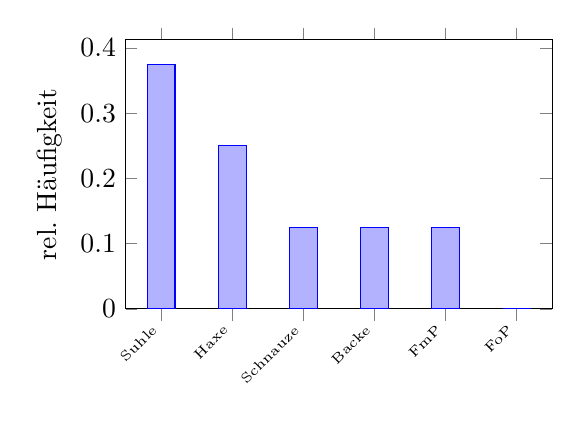
\begin{tikzpicture}
            \begin{axis}[
                ybar, width=7cm, height=5cm,
                symbolic x coords={Suhle,Haxe,Schnauze,Backe,FmP,FoP},
                xtick=data, x tick label style={rotate=45,anchor=east,font=\tiny},
                ylabel={rel.\ Häufigkeit}, ymin=0,
                bar width=10pt
            ]
                \addplot coordinates {(Suhle,0.375) (Haxe,0.25) (Schnauze,0.125) (Backe,0.125) (FmP,0.125) (FoP,0)};
            \end{axis}
        \end{tikzpicture}
        \caption{Balkendiagramm --- kleiner Datensatz}
    \end{subfigure}
    \hfill
    \begin{subfigure}[t]{0.48\textwidth}
        \centering
        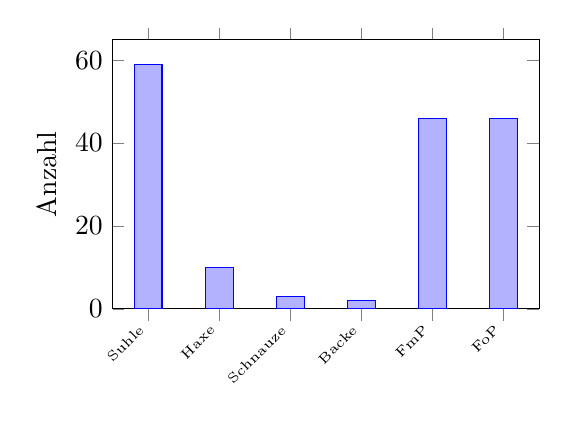
\begin{tikzpicture}
            \begin{axis}[
                ybar, width=7cm, height=5cm,
                symbolic x coords={Suhle,Haxe,Schnauze,Backe,FmP,FoP},
                xtick=data, x tick label style={rotate=45,anchor=east,font=\tiny},
                ylabel={Anzahl}, ymin=0,
                bar width=10pt
            ]
                \addplot coordinates {(Suhle,59) (Haxe,10) (Schnauze,3) (Backe,2) (FmP,46) (FoP,46)};
            \end{axis}
        \end{tikzpicture}
        \caption{Balkendiagramm --- Experiment vom 14.01.2026}
    \end{subfigure}\label{fig:figure5}
\end{figure}


\begin{bsp}[\gls{Merkmal}e treten in verschiedenen Ausprägungen auf]
    \txc{(Skript 26)}
    \begin{mytable}
        \begin{tabular}{|l|l| p{8cm}|}
            \hline
            \textbf{Versuchseinheit} & \textbf{Merkmal}              & \textbf{Ausprägung}                                           \\
            \hline
            Schweinchen              & Lage                          & Suhle, Haxe, Schnauze, Backe, Faul-mit-Punkt, Faul-ohne-Punkt \\
            Schweinchen              & Farbe                         & weiß, braun, rosa, schwarz                                    \\
            Studierende              & erster Buchstabe vom Vornamen & A,\dots,Z                                                     \\
            & Geburtstag                    & $1,\dots,365$                                                 \\
            & Abiturnote                    & $x/10$ mit $x\in\{10,\dots,40\}$                              \\
            Schüler                  & Alter in Jahren               & $n\in\nz$                                                     \\
            & Größe                         & $l\in(0,\infty)$                                              \\
            & Gewicht                       & untergewichtig, normal, übergewichtig                         \\
            \hline
        \end{tabular}
    \end{mytable}
\end{bsp}

\begin{defi}[Arten von Merkmalen]
    \txc{(Skript 26)} \\
    Für quantitative \gls{Merkmal}e unterscheiden wir zwischen \emph{diskreten} und \emph{stetigen} \gls{Merkmal}en (vgl.\ Alter in Jahren mit Größe).

    Für qualitative \gls{Merkmal}e unterscheiden wir zwischen \emph{ordinalen} \gls{Merkmal}en bzw.\ \emph{Rangmerkmalen} einerseits und \emph{nominalen} \gls{Merkmal}en andererseits.
    Rangmerkmale weisen im Gegensatz zu nominalen \gls{Merkmal}en eine natürliche Ordnung auf (vgl.\ untergewichtig, normal, übergewichtig mit weiß, braun, rosa, schwarz).
\end{defi}
% TODO welche arten von merkmalen gibt es?

\definstat{Grundgesamtheit}

Die \gls{Grundgesamtheit} muss bei jeder \gls{Datenerhebung} sorgfältig definiert werden.

\begin{mytable}
    \begin{tabular}{lll}
        \hline
        \textbf{Versuchseinheit} & \textbf{Merkmal}              & \textbf{Grundgesamtheit}                      \\
        \hline
        Schweinchen              & Lage                          & alle vorhandenen Schweinchen nach dem Würfeln \\
        Schweinchen              & Farbe                         & alle Schweinchen im Beutel                    \\
        Studierende              & erster Buchstabe vom Vornamen & alle Studierenden im Hörsaal                  \\
        & Geburtstag                    &                                               \\
        & Abiturnote                    &                                               \\
        Schüler                  & Alter in Jahren               & alle Schüler einer Jahrgangsstufe             \\
        & Größe                         &                                               \\
        & Gewicht                       &                                               \\
        \hline
    \end{tabular}
\end{mytable}

\textbf{Stichprobe:} Die \gls{Grundgesamtheit} ist oft zu groß, um komplett ausgewertet zu werden.
In der Regel wird daher nur eine Stichprobe ausgewertet.

\definstat{StichprobeN}

Dabei wird, leicht missbräuchlich, in der Regel nicht unterschieden zwischen den $n$ \gls{Versuchseinheit}en, die
für die Stichprobe aus der \gls{Grundgesamtheit} gewählt werden, und den zu der Stichprobe gehörenden \gls{Merkmal}sausprägungen.

\definstat{Urliste}


\begin{bsp}
    \txc{(Skript 26)} \\
    \begin{mytable}
        \begin{tabular}{ll}
            \hline
            \textbf{Versuchseinheit} & \textbf{Merkmalsausprägung} \\
            \hline
            Schweinchen 1            & Suhle                       \\
            Schweinchen 2            & Schnauze                    \\
            Schweinchen 3            & Faul-mit-Punkt              \\
            Schweinchen 4            & Haxe                        \\
            Schweinchen 5            & Backe                       \\
            Schweinchen 6            & Haxe                        \\
            Schweinchen 7            & Suhle                       \\
            Schweinchen 8            & Suhle                       \\
            \hline
        \end{tabular}
    \end{mytable}

    Kürzere Darstellung als Liste:
    \[
        (1,\text{Suhle}),(2,\text{Schnauze}),(3,\text{Faul-mit-Punkt}),(4,\text{Haxe}),(5,\text{Backe}),(6,\text{Haxe}),(7,\text{Suhle}),(8,\text{Suhle})
    \]
\end{bsp}

\begin{defi}[\gls{Häufigkeitsverteilung}]
    \txc{(Skript 26)} \\
    Gegeben: Stichprobe $x_1,\dots,x_n$; \gls{Merkmal} $X$ mit genau $s$ möglichen Ausprägungen $a_1,\dots,a_s$.
    \begin{enumerate}[label=(\alph*)]
        \item \textbf{Absolute Häufigkeit} der Ausprägung $a_i$ in der Stichprobe $x_1,\dots,x_n$:
        \[
            H_n(a_i) = \#\{j\in\{1,\dots,n\} : x_j = a_i\}
        \]
        \item \textbf{Absolute empirische \gls{Häufigkeitsverteilung}} der Stichprobe $x_1,\dots,x_n$:
        Abbildung $H_n : \{a_1,\dots,a_s\}\to\{0,\dots,n\}$ mit $a_i\mapsto H_n(a_i)$ für $i=1,\dots,s$.
        \item \textbf{Relative Häufigkeit} der Ausprägung $a_i$ in der Stichprobe $x_1,\dots,x_n$:
        \[
            h_n(a_i) = \frac{1}{n} H_n(a_i)
        \]
        \item \textbf{Relative \gls{Häufigkeitsverteilung}} der Stichprobe $x_1,\dots,x_n$:
        Abbildung $h_n : \{a_1,\dots,a_s\}\to\left\{\frac{k}{n} : k\in\{0,\dots,n\}\right\}$ mit $a_i\mapsto h_n(a_i)$ für $i=1,\dots,s$.
    \end{enumerate}
\end{defi}

\begin{bem}
    \[
        H_n(a_1)+\cdots+H_n(a_s) = n \qquad\text{und}\qquad h_n(a_1)+\cdots+h_n(a_s)=1
    \]
\end{bem}

\begin{bsp}[Werfen von acht Schweinchen]
    \label{bsp:acht-schweinchen}  \txc{(Skript 26)} \\
    Stichprobe: Suhle, Schnauze, Faul-mit-Punkt, Haxe, Backe, Haxe, Suhle, Suhle

    bzw.\ Urliste: $(1,\text{Suhle}),(2,\text{Schnauze}),(3,\text{Faul-mit-Punkt}),(4,\text{Haxe}),(5,\text{Backe}),(6,\text{Haxe}),(7,\text{Suhle}),(8,\text{Suhle})$

    \begin{mytable}
        \begin{tabular}{lcc}
            \hline
            \textbf{Merkmalsausprägung} & $H_n(a_i)$ & $h_n(a_i)$ \\
            \hline
            Suhle                       & 3          & $3/8$      \\
            Haxe                        & 2          & $1/4$      \\
            Schnauze                    & 1          & $1/8$      \\
            Backe                       & 1          & $1/8$      \\
            Faul-mit-Punkt              & 1          & $1/8$      \\
            Faul-ohne-Punkt             & 0          & $0$        \\
            \hline
        \end{tabular}
    \end{mytable}
\end{bsp}

\subsection{Graphische Darstellungen eindimensionaler Daten}\label{subsec:graphische-darstellungen-eindimensionaler-daten}


Für den kleinen Datensatz (Beispiel \autoref{bsp:acht-schweinchen}) und den großen Datensatz (aus der Vorlesung vom 14.01.2026) mit den
Schweinchen haben wir u.a.\ folgende Möglichkeiten der graphischen Darstellung: Kreis- bzw.\ Tortendiagramm sowie Stab- bzw.\ Balkendiagramm (siehe Abbildungen oben).

\begin{bsp}[Alter von Berufstätigen]
    \txc{(Skript 26)}
    \[
        \begin{array}{l}
            21, 22, 24, 28, 28, 28, 32, 32, 33, 35,\\
            35, 36, 37, 37, 37, 40, 40, 41, 43, 43,\\
            44, 47, 48, 48, 53, 53, 53, 58, 60, 60,\\
            24, 25, 26, 27, 27, 27, 27, 28, 29, 31,\\
            31, 31, 31, 32, 33, 33, 34, 34, 35, 35,\\
            35, 36, 36, 36, 36, 37, 37, 37, 37, 38,\\
            38, 39, 39, 39, 39, 41, 41, 41, 41, 42,\\
            42, 42, 45, 45, 45, 46, 47, 47, 47, 48,\\
            49, 49, 49, 52, 52, 52, 54, 54, 55, 55,\\
            55, 56, 57, 61, 64, 65, 65, 65, 65, 65
        \end{array}
    \]
    (Simulierte Daten, bereits der Größe nach geordnet, mit Stichprobengröße $n=100$.)

    \begin{mytable}
        \small
        \begin{tabular}{l*{20}{c}}
            \hline
            Alter & 18 & 19 & 20 & 21 & 22 & 23 & 24 & 25 & 26 & 27 & 28 & 29 & 30 & 31 & 32 & 33 & 34 & 35 & 36 & 37 \\
            Anz.
            & 0  & 0  & 0  & 1  & 1  & 0  & 2  & 1  & 1  & 4  & 4  & 1  & 0  & 4  & 3  & 3  & 2  & 5  & 5  & 7  \\
            \hline
            Alter & 38 & 39 & 40 & 41 & 42 & 43 & 44 & 45 & 46 & 47 & 48 & 49 & 50 & 51 & 52 & 53 & 54 & 55 & 56 & 57 \\
            Anz.
            & 2  & 4  & 2  & 5  & 3  & 2  & 1  & 3  & 1  & 4  & 3  & 3  & 0  & 0  & 3  & 3  & 2  & 3  & 1  & 1  \\
            \hline
            Alter & 58 & 59 & 60 & 61 & 62 & 63 & 64 & 65 & 66 & 67 &    &    &    &    &    &    &    &    &    &    \\
            Anz.
            & 1  & 0  & 2  & 1  & 0  & 0  & 1  & 5  & 0  & 0  &    &    &    &    &    &    &    &    &    &    \\
            \hline
        \end{tabular}
    \end{mytable}

    Weder Balken- noch Kreisdiagramm sind sinnvoll bei so vielen verschiedenen Ausprägungen:

    \begin{figure}[H]
        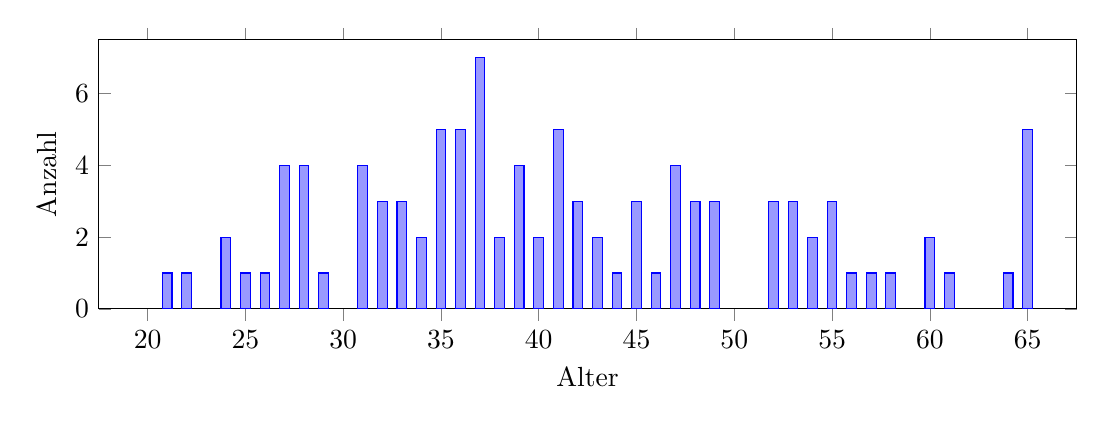
\begin{tikzpicture}
            \begin{axis}[
                ybar, width=14cm, height=5cm,
                xlabel={Alter}, ylabel={Anzahl}, ymin=0, ymax=7.5,
                xmin=17.5, xmax=67.5, bar width=3.5pt,
                xtick={20,25,...,65}
            ]
                \addplot+[fill=blue!40] coordinates {
                    (21,1)(22,1)(24,2)(25,1)(26,1)(27,4)(28,4)(29,1)(31,4)(32,3)(33,3)(34,2)(35,5)(36,5)(37,7)
                    (38,2)(39,4)(40,2)(41,5)(42,3)(43,2)(44,1)(45,3)(46,1)(47,4)(48,3)(49,3)(52,3)(53,3)(54,2)
                    (55,3)(56,1)(57,1)(58,1)(60,2)(61,1)(64,1)(65,5)
                };
            \end{axis}
        \end{tikzpicture}\label{fig:figure10}
    \end{figure}

    \paragraph{Histogramm}
    Klasseneinteilung wählen: Jede Klasse möge 5 Jahre erfassen -- aber stimmt das am Rand?

    \begin{mytable}
        \begin{tabular}{l*{11}{c}}
            \hline
            Alter & $\leq 19$ & 20--24 & 25--29 & 30--34 & 35--39 & 40--44 & 45--49 & 50--54 & 55--59 & 60--64 & $\geq 65$ \\
            Anz.
            & 0         & 4      & 11     & 12     & 23     & 13     & 14     & 8      & 6      & 4      & 5         \\
            \hline
        \end{tabular}
    \end{mytable}

    \begin{figure}[H]
        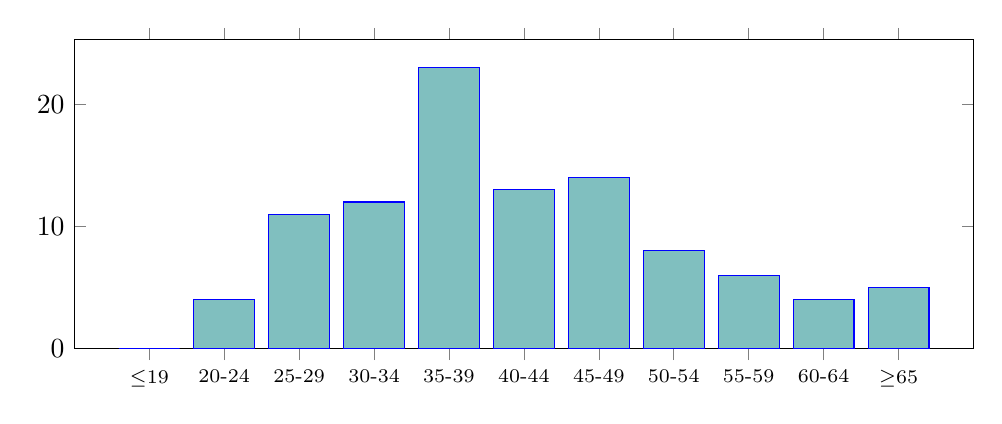
\begin{tikzpicture}
            \begin{axis}
                [
                ybar, width=13cm, height=5.5cm, ymin=0,
                symbolic x coords={$\leq$19,20-24,25-29,30-34,35-39,40-44,45-49,50-54,55-59,60-64,$\geq$65},
                xtick=data, x tick label style={font=\scriptsize},
                bar width=22pt
                ]
                \addplot+[fill=teal!50] coordinates {
                    ($\leq$19,0) (20-24,4) (25-29,11) (30-34,12) (35-39,23) (40-44,13) (45-49,14) (50-54,8) (55-59,6) (60-64,4) ($\geq$65,5)
                };
            \end{axis}
        \end{tikzpicture}\label{fig:figure9}
    \end{figure}

    Wenn als Alter zum Beispiel nur Werte im Bereich 18--67 auftreten können, sollte die Breite der Randbalken angepasst werden (schmalere Klassen ``18--19'' und ``65--67'').
\end{bsp}

\begin{bem}[Restklasse]
    Sollte es Ausreißer in den Daten geben (z.B.\ einen Berufstätigen im Alter von 91 Jahren), so wird eine Restklasse gebildet.
    Für diese wird kein Balken gezeichnet, sondern nur vermerkt, wie viele Elemente sie hat.
\end{bem}

Es gibt weitere übliche Darstellungen wie das Stamm-Blatt-Diagramm oder den Box-Plot.
Wir verweisen diesbezüglich auf die Literatur.


\section{Empirische Häufigkeitsverteilungen und ihre Lagemaße}\label{sec:empirische-haufigkeitsverteilungen-und-ihre-lagemae}

\noindent \textbf{Ziel:} Charakterisierung von \gls{Häufigkeitsverteilung}en durch Kennzahlen.

\noindent \textbf{Gegeben:} Stichprobe $x_1,\dots,x_n$ eines eindimensionalen \gls{Merkmal}s $X$.

\begin{defi}[\gls{Lagemaß}]
    \label{def:lagemaß}  \txc{(Skript 26)} \\
    Sei $X$ ein quantitatives \gls{Merkmal}.
    Eine Funktion $l:\rz^n\to\rz$, $(x_1,\dots,x_n)\mapsto l(x_1,\dots,x_n)$, heißt \emph{Lagemaß}, wenn
    \[
        l(x_1+a,\dots,x_n+a) = l(x_1,\dots,x_n) + a \qquad \forall (x_1,\dots,x_n)\in\rz^n \ \forall a\in\rz \cdot
    \]
    Anschaulich bedeutet das, dass ein Verschieben der Werte der Stichprobe um $a$ äquivalent ist zum Verschieben des \gls{Lagemaß}es um $a$.
\end{defi}


\begin{kom}[Andere Definitionen von Lagemaß]
    \paragraph{Wikipedia:}  Ein Lagemaß oder Lageparameter ist in der Stochastik eine Kennzahl der Verteilung einer Zufallsvariable beziehungsweise
    eines Wahrscheinlichkeitsmaßes.
    Anschaulich ist es die Aufgabe eines Lagemaßes, den ``typischen'' Wert einer Zufallsvariable anzugeben.


    % \href{https://bjoernwalther.com/lagemasse-in-der-statistik/}{Björn Walther}

    \paragraph{Björn Walther:} Lagemaße (auch Lageparameter) sind Kennzahlen, die
    im Rahmen der deskriptiven Statistik genutzt werden.
    Sie treffen eine Aussage über die zentrale Tendenz von Variablen im Datensatz.
    Mit ihnen ist also erkennbar, wo in der Stichprobe die ``Musik spielt''.

    % \href{https://welt-der-bwl.de/Lagema%C3%9Fe}{Welt der BWL}

    \paragraph{Welt der BWL:} Lagemaße der Statistik – auch Maße der zentralen Tendenz genannt – geben an, was in einer Datenmenge das Zentrum bzw. der Schwerpunkt ist, zum Beispiel der häufigste Wert oder der Durchschnitt.

    % \href{https://studyflix.de/statistik/deskriptive-statistik-1052}{studyflix}

    \paragraph{studyflix} Lageparameter geben die zentrale Tendenz des Datensatzes an.
    Konkret wird also untersucht, ob die gemessenen Werte eher groß oder klein sind.
    Bei einer Umfrage kann man beispielsweise ermitteln, ob eher jüngere oder ältere Menschen befragt wurden.
\end{kom}

\begin{bsp}[\defirefman{lagemaß}]
    \begin{itemize}
        \item Das \emph{arithmetische Mittel} $\bar x = \frac{1}{n}\sum_{i=1}^n x_i$ der Stichprobe $x_1,\dots,x_n$ ist ein \gls{Lagemaß}.
        \item Das \emph{geometrische Mittel} $\bar x_g = \sqrt[n]{x_1\cdots x_n}$ der Stichprobe $x_1,\dots,x_n$ ist \emph{kein} \gls{Lagemaß}.
        \item Das \emph{harmonische Mittel} $\bar x_h = \dfrac{n}{\frac{1}{x_1}+\cdots+\frac{1}{x_n}}$ der Stichprobe $x_1,\dots,x_n$ ist \emph{kein} \gls{Lagemaß}.
    \end{itemize}

    \noindent Wir wollen diese Aussagen beweisen.

    \smallskip

    \paragraph{Beweis - Das arithmetische Mittel $\bar x=\frac{1}{n}\sum_{i=1}^n x_i$ ist ein Lagemaß:}

    Sei $l_{\mathrm{arith}}(x_1,\dots,x_n) = \frac1n\sum_{i=1}^n x_i$.
    Dann gilt für alle $(x_1,\dots,x_n)\in\rz^n$ und alle $a\in\rz$
    \[
        l_{\mathrm{arith}}(x_1+a,\dots,x_n+a) = \frac1n \sum_{i=1}^n [x_i+a] = \frac1n\sum_{i=1}^n x_i + \frac1n\sum_{i=1}^n a = l_{\mathrm{arith}}(x_1,\dots,x_n) + a \cdot
    \]

    \smallskip

    \paragraph{Beweis - Das geometrische Mittel $\bar x_g = \sqrt[n]{x_1\cdots x_n}$ ist kein Lagemaß:}

    Beachte zunächst, dass das geometrische Mittel nur für $x_1,\dots,x_n\geq 0$ sinnvoll definiert ist.
    Auch wenn wir nur $x_1,\dots,x_n\geq 0$ und $a>0$ betrachten, erfüllt das geometrische Mittel nicht die Anforderung an ein \gls{Lagemaß}:

    Seien $n=2$ und $l_g(x_1,x_2)=\sqrt{x_1\cdot x_2}$.
    Wäre $l_g$ ein \gls{Lagemaß}, so müsste gelten
    \[
        (*) \qquad l_g(x_1+a,x_2+a) = l_g(x_1,x_2)+a \qquad \forall (x_1,x_2)\in\rz^2 \ \forall a\in\rz \cdot
    \]
    Quadrieren beider Seiten zeigt, dass $(*)$ äquivalent ist zu $\sqrt{x_1\cdot x_2} = \frac{x_1+x_2}{2}$.
    Das heißt, dass das geometrische Mittel nur dann ein \gls{Lagemaß} sein kann, wenn arithmetisches und geometrisches Mittel für alle $(x_1,x_2)\in\rz^2$ gleich wären.

    \smallskip

    \paragraph{Beweis - Das harmonische Mittel $\bar x_h = \dfrac{n}{\frac1{x_1}+\cdots+\frac1{x_n}}$ ist kein Lagemaß:}

    Beachte zunächst, dass das harmonische Mittel nur für $x_1,\dots,x_n\neq 0$ sinnvoll definiert ist.
    Selbst wenn wir nur $x_1,\dots,x_n>0$ und $a>0$ betrachten, erfüllt das harmonische Mittel nicht die Anforderung an ein \gls{Lagemaß}:

    Seien $n=2$ und $l_h(x_1,x_2) = \dfrac{2}{1/x_1+1/x_2}$.
    Die Wahl $x_1=1$, $x_2=2$ und $a=1$ zeigt
    \[
        l_h(x_1+a,x_2+a) = \frac{2}{\frac1{1+1}+\frac1{2+1}} = \frac{12}{5}
        \qquad\text{und}\qquad
        l_h(x_1,x_2)+a = \frac{2}{\frac11+\frac12}+1 = \frac73 ,
    \]
    also $l_h(x_1+a,x_2+a)\neq l_h(x_1,x_2)+a$.
\end{bsp}

\begin{bsp}[10$\times$ Würfeln]
    \txc{(Skript 26)} \\
    Stichprobe $6,2,5,4,1,6,5,4,5,4$ der Länge $n=10$.

    \begin{figure}[H]
        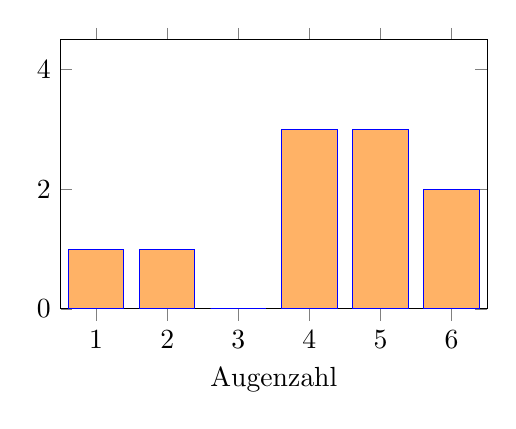
\begin{tikzpicture}
            \begin{axis}[ybar, width=7cm, height=5cm, xtick=data, ymin=0, ymax=4.5, bar width=20pt, xlabel={Augenzahl}]
                \addplot+[fill=orange!60] coordinates {(1,1)(2,1)(3,0)(4,3)(5,3)(6,2)};
            \end{axis}
        \end{tikzpicture}\label{fig:figure8}
    \end{figure}

    \begin{itemize}
        \item Arithmetisches Mittel $\bar x = \frac1n\sum_{i=1}^n x_i = \frac1{10}[6+2+5+4+1+6+5+4+5+4] = 4.2$
        \item Geometrisches Mittel $\bar x_g = \sqrt[n]{x_1\cdots x_n} = \sqrt[10]{6\cdot2\cdot5\cdot4\cdot1\cdot6\cdot5\cdot4\cdot5\cdot4} \approx 3.77$
        \item Harmonisches Mittel $\bar x_h = \dfrac{n}{\frac1{x_1}+\cdots+\frac1{x_n}} = \dfrac{10}{\frac16+\frac12+\frac15+\frac14+\frac11+\frac16+\frac15+\frac14+\frac15+\frac14} \approx 3.14$
    \end{itemize}
\end{bsp}

\begin{satz}[Eigenschaften des arithmetischen Mittels]
    \txc{(Skript 26)} \\
    \begin{enumerate}[label=(\alph*)]
        \item \textbf{Schwerpunkteigenschaft:}
        \txc{Die Schwerpunkteigenschaft (auch Nulleigenschaft genannt) besagt, dass die Summe der scheinbaren Fehler bzw. die Summe der Abweichungen aller beobachteten Messwerte vom arithmetischen Mittel gleich Null ist. Also:}
        % https://de.wikipedia.org/wiki/Arithmetisches_Mittel
        \[
            \sum_{i=1}^n (x_i-\bar x) = 0
        \]
        \item \textbf{Minimierungseigenschaft:} $\displaystyle\sum_{i=1}^n (x_i-c)^2 \to \min$ für $c=\bar x$.

        Das arithmetische Mittel minimiert die quadratische Abweichung der Stichprobenwerte von einer Konstanten $c\in\rz$:
        \[
            \sum_{i=1}^n (x_i-\bar x)^2 = \inf_{c\in\rz} \sum_{i=1}^n (x_i-c)^2
        \]
    \end{enumerate}

    \paragraph{Beweis.}
    \begin{enumerate}[label=(\alph*)]
        \item Linearität der Summe und die Definition von $\bar x$ zeigen, dass
        \[
            \sum_{i=1}^n (x_i-\bar x) = \sum_{i=1}^n x_i - \sum_{i=1}^n \bar x = \sum_{i=1}^n x_i - n\cdot\frac1n\sum_{i=1}^n x_i = 0 \cdot
        \]
        \item Eine Nullergänzung und Ausquadrieren zeigen, dass
        \[
            \sum_{i=1}^n (x_i-c)^2 = \sum_{i=1}^n \big[(x_i-\bar x)+(\bar x-c)\big]^2 = \sum_{i=1}^n (x_i-\bar x)^2 + 2(\bar x-c)\sum_{i=1}^n (x_i-\bar x) + n(\bar x-c)^2 \cdot
        \]
        Der erste Summand auf der rechten Seite hängt nicht von $c$ ab.
        Der zweite Summand ist gleich Null aufgrund der Schwerpunkteigenschaft.
        Der dritte Summand ist stets nichtnegativ und gleich Null genau dann, wenn $c=\bar x$ ist.
        Somit wird
        \[
            \sum_{i=1}^n (x_i-c)^2 = \sum_{i=1}^n (x_i-\bar x)^2 + n(\bar x-c)^2
        \]
        minimal für $c=\bar x$ mit Wert $\sum_{i=1}^n (x_i-\bar x)^2$. \qedhere
    \end{enumerate}
\end{satz}




\begin{defi}[Modalwert / Modus]
    \txc{(Skript 26)} \\
    Sei $X$ ein beliebiges eindimensionales \gls{Merkmal} ($X$ kann nominal sein) mit Ausprägungen $a_1,\dots,a_s$.
    Eine Ausprägung $a$ des \gls{Merkmal}s $X$ heißt \emph{Modalwert} oder \emph{Modus}, wenn
    \[
        H_n(a) \geq H_n(x_i) \qquad \forall i=1,\dots,n \cdot
    \]
    \txc{Also wenn die Ausprägung $a$ die größte Häufigkeit hat. Also der Modalwert der Wert, der in der Stichprobe am häufigsten vorkommt.}
    % https://de.wikipedia.org/wiki/Modus_(Statistik)
\end{defi}

\begin{bem}
    \txc{(Skript 26)} \\
    \begin{enumerate}[label=(\alph*)]
        \item $a$ ist genau dann ein Modalwert, wenn keine andere Ausprägung in der Stichprobe häufiger auftritt als $a$.
        \item Der Modalwert ist in der Regel nicht eindeutig, siehe folgendes Beispiel.
        \item $H_n(a)\geq H_n(x_i)\ \forall i=1,\dots,n \iff H_n(a)\geq H_n(a_k)\ \forall k=1,\dots,s$.
        \item Für quantitative \gls{Merkmal}e ist der Modalwert ein \gls{Lagemaß}.
    \end{enumerate}
\end{bem}

\begin{defi}[Unimodal]
    \txc{(Skript 26)} \\
    Wir schreiben $x_{\mathrm{mod}}$ für den Modalwert einer Stichprobe, sofern dieser eindeutig bestimmt ist.
    In diesem Fall heißen die Häufigkeitsverteilungen $H_n$ und $h_n$ \emph{unimodal}.

    \txc{Umgangssprachlich: Unimodalität bedeutet, dass es nur einen einzigen Höchstwert (Modalwert / Modus) gibt.}
\end{defi}

\begin{bsp}[Würfeln]
    \txc{(Skript 26)} \\
    \begin{figure}[H]
        \begin{subfigure}[t]{0.48\textwidth}
            \centering
            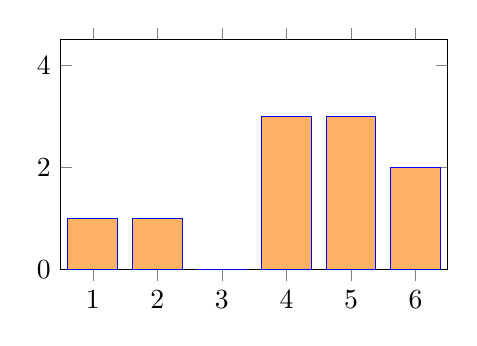
\begin{tikzpicture}
                \begin{axis}[ybar, width=6.5cm, height=4.5cm, xtick=data, ymin=0, ymax=4.5, bar width=18pt]
                    \addplot+[fill=orange!60] coordinates {(1,1)(2,1)(3,0)(4,3)(5,3)(6,2)};
                \end{axis}
            \end{tikzpicture}\\
            \footnotesize Stichprobe $6,2,5,4,1,6,5,4,5,4$, $n=10$\\
            Modalwerte $4$ und $5$ --- \emph{nicht} unimodal
        \end{subfigure}
        \hfill
        \begin{subfigure}[t]{0.48\textwidth}
            \centering
            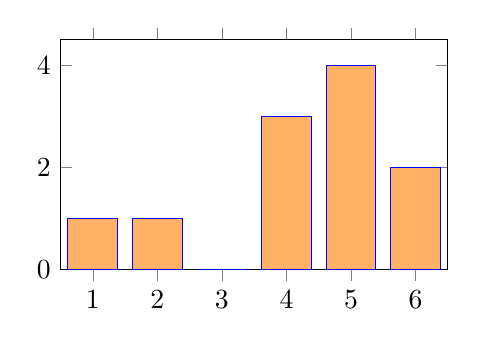
\begin{tikzpicture}
                \begin{axis}[ybar, width=6.5cm, height=4.5cm, xtick=data, ymin=0, ymax=4.5, bar width=18pt]
                    \addplot+[fill=orange!60] coordinates {(1,1)(2,1)(3,0)(4,3)(5,4)(6,2)};
                \end{axis}
            \end{tikzpicture}\\
            \footnotesize Stichprobe $6,2,5,4,1,6,5,4,5,4,5$, $n=11$\\
            Modalwert $x_{\mathrm{mod}}=5$ --- unimodal
        \end{subfigure}\label{fig:figure7}
    \end{figure}
\end{bsp}

\begin{defi}[Median / Zentralwert]
    \txc{(Skript 26)} \\
    Sei $X$ ein quantitatives \gls{Merkmal}.
    Ist die Stichprobe $x_1,\dots,x_n$ gegeben, so schreiben wir $x_{(1)},\dots,x_{(n)}$ für die \emph{geordnete Stichprobe}, d.h.\ es gelten
    \[
        \{x_1,\dots,x_n\} = \{x_{(1)},\dots,x_{(n)}\} \qquad\text{und}\qquad x_{(1)}\leq\cdots\leq x_{(n)} \cdot
    \]
    Der \emph{Median} oder \emph{Zentralwert} ist definiert durch
    \[
        x_{\mathrm{med}} =
        \begin{cases}
            x_{\left(\frac{n+1}{2}\right)} & \text{falls } n \text{ ungerade ist,}\\[1ex]
            \dfrac12\left[x_{\left(\frac n2\right)} + x_{\left(\frac n2+1\right)}\right] & \text{falls } n \text{ gerade ist.}
        \end{cases}
    \]
\end{defi}

\begin{bsp}[Würfeln]
    \txc{(Skript 26)} \\
    \begin{mytable}
        \begin{minipage}{0.48\textwidth}
            \centering
            Stichprobe $6,2,5,4,1,6,5,4,5,4$\\
            geordnet $1,2,4,4,4,5,5,5,6,6$, $n=10$
            \[
                x_{\mathrm{med}} = \frac12\left[x_{(5)}+x_{(6)}\right] = \frac{4+5}{2} = 4.5
            \]
        \end{minipage}
        \hfill
        \begin{minipage}{0.48\textwidth}
            \centering
            Stichprobe $6,2,5,4,1,6,5,4,5,4,5$\\
            geordnet $1,2,4,4,4,5,5,5,5,6,6$, $n=11$
            \[
                x_{\mathrm{med}} = x_{(6)} = 5
            \]
        \end{minipage}
    \end{mytable}
\end{bsp}

\begin{satz}[Eigenschaften des Medians]
    \label{satz:median_eigenschaften} \txc{(Skript 26)} \\
    \begin{enumerate}[label=(\alph*)]
        \item Der Median ist ein \gls{Lagemaß}.
        \item Der Median $x_{\mathrm{med}}$ erfüllt
        \[
            \sum_{\substack{k=1:\\ a_k\leq x_{\mathrm{med}}}}^s h_n(a_k) \geq \frac12
            \qquad\text{und}\qquad
            \sum_{\substack{k=1:\\ a_k\geq x_{\mathrm{med}}}}^s h_n(a_k) \geq \frac12 \cdot
        \]
        Das heißt, mindestens die Hälfte der Werte in der Stichprobe sind kleiner oder gleich dem Wert des Medians und mindestens die Hälfte der Werte in der Stichprobe sind größer oder gleich dem Wert des Medians.
        \item Gelten
        \[
            \sum_{\substack{k=1:\\ a_k\leq a}}^s h_n(a_k)\geq\frac12 \qquad\text{und}\qquad \sum_{\substack{k=1:\\ a_k\geq a}}^s h_n(a_k)\geq\frac12 \qquad\text{für ein } a\in\rz ,
        \]
        so folgt $x_{(\lceil n/2\rceil)} \leq a \leq x_{(\lceil n/2\rceil+1)}$.
        Dabei muss $a$ keine Ausprägung des \gls{Merkmal}s $X$ sein.
        \item \textbf{Minimierungseigenschaft:} \txc{Der Median minimiert die absoluten Abweichungen}
        \[
            \sum_{i=1}^n |x_i-c| \to \min \qquad \text{für ein } c\in\left[x_{\left(\lfloor\frac{n+1}2\rfloor\right)}, x_{\left(\lceil\frac{n+1}2\rceil\right)}\right] \cdot
        \]
    \end{enumerate}

    \paragraph{Beweis.}
    \begin{enumerate}[label=(\alph*)]
        \item Können Sie diese Aussage selbst beweisen?
        \item Zu zeigen ist, dass der Median $\sum_{k=1: a_k\leq x_{\mathrm{med}}}^s h_n(a_k)\geq\frac12$ und $\sum_{k=1: a_k\geq x_{\mathrm{med}}}^s h_n(a_k)\geq\frac12$ erfüllt.
        Wir begnügen uns damit, die erste Aussage zu zeigen; die zweite lässt sich analog beweisen.

        Unter Verwendung der Definition der absoluten empirischen Häufigkeitsverteilung sehen wir, dass
        \[
            \sum_{\substack{k=1:\\ a_k\leq x_{\mathrm{med}}}}^s h_n(a_k)
            = \frac1n \sum_{\substack{k=1:\\ a_k\leq x_{\mathrm{med}}}}^s H_n(a_k)
            = \frac1n \#\{i\in\{1,\dots,n\}: x_i\leq x_{\mathrm{med}}\}
            = \frac1n \#\{i\in\{1,\dots,n\}: x_{(i)}\leq x_{\mathrm{med}}\} \cdot
        \]

        \textbf{1.\ Fall: $n$ ungerade.} Für ungerade $n$ ist $x_{\mathrm{med}}=x_{\left(\frac{n+1}2\right)}$, und daher
        \[
            \#\{i\in\{1,\dots,n\}: x_{(i)}\leq x_{\mathrm{med}}\} \geq \frac{n+1}{2} \geq \frac n2 ,
        \]
        weil mindestens die $\frac{n+1}2$ Elemente $x_{(1)}\leq\cdots\leq x_{\left(\frac{n+1}2\right)}$ in der Menge sind.
        Daraus folgt die Behauptung.

        Beispiel: $n=5$, geordnete Stichprobe $1,1,2,2,5$ (Augenzahl beim Würfeln).
        Es ist $x_{\mathrm{med}}=x_{(3)}=2$, und
        $\frac15\#\{i: x_{(i)}\leq 2\} = \frac45\geq\frac12$, ebenso $\sum_{k: a_k\leq x_{\mathrm{med}}} h_5(a_k) = h_5(1)+h_5(2)=\frac25+\frac25=\frac45\geq\frac12$.

        \textbf{2.\ Fall: $n$ gerade.} Für gerade $n$ ist $x_{\mathrm{med}}=\frac12\left[x_{\left(\frac n2\right)}+x_{\left(\frac n2+1\right)}\right]\geq x_{\left(\frac n2\right)}$, weil $x_{\left(\frac n2+1\right)}\geq x_{\left(\frac n2\right)}$.
        Daher gilt
        $\#\{i: x_{(i)}\leq x_{\mathrm{med}}\}\geq \frac n2$, weil mindestens die $\frac n2$ Elemente $x_{(1)}\leq\cdots\leq x_{\left(\frac n2\right)}$ in der Menge sind.

        Beispiel: $n=6$, geordnete Stichprobe $1,1,1,2,2,5$.
        Es ist $x_{\mathrm{med}}=\frac12[x_{(3)}+x_{(4)}]=\frac32$, und
        $\frac16\#\{i: x_{(i)}\leq \frac32\} = \frac36=\frac12\geq\frac12$, ebenso $h_6(1)=\frac36=\frac12\geq\frac12$.

        \item Wir müssen zeigen: Gelten $\sum_{k: a_k\leq a} h_n(a_k)\geq\frac12$ und $\sum_{k: a_k\geq a} h_n(a_k)\geq\frac12$ für ein $a\in\rz$, so folgt $x_{(\lceil n/2\rceil)}\leq a\leq x_{(\lceil n/2+1\rceil)}$.

        Wir schreiben wieder die Summen um und erhalten $\#\{i: x_{(i)}\leq a\}\geq\frac n2$ und $\#\{i: x_{(i)}\geq a\}\geq\frac n2$.

        \textbf{1.\ Fall: $n$ ungerade.} Für ungerade $n$ ist $\frac n2\notin\nz$.
        Daher müssen sogar $\#\{i: x_{(i)}\leq a\}\geq\frac{n+1}2$ und $\#\{i: x_{(i)}\geq a\}\geq\frac{n+1}2$ gelten.
        Folglich ergibt sich durch Abzählen von unten bzw.\ oben, dass $x_{(1)}\leq\cdots\leq x_{\left(\frac{n+1}2\right)}\leq a$ und $x_{(n)}\geq\cdots\geq x_{\left(\frac{n+1}2\right)}\geq a$ gelten.
        Damit haben wir sogar $x_{\mathrm{med}}=x_{\left(\frac{n+1}2\right)}=a$ gezeigt.

        Beispiel: $n=5$, geordnete Stichprobe $1,1,2,2,5$.
        Es gilt $h_5(1)=\frac25<\frac12$, aber $h_5(1)+h_5(2)\geq\frac12$; ebenso von oben betrachtet muss $a=2$ gelten.

        \textbf{2.\ Fall: $n$ gerade.} Für gerade $n$ wissen wir nur $\#\{i: x_{(i)}\leq a\}\geq\frac n2$ und $\#\{i: x_{(i)}\geq a\}\geq\frac n2$.
        Wieder ergibt sich $x_{(1)}\leq\cdots\leq x_{\left(\frac n2\right)}\leq a$ und $x_{(n)}\geq\cdots\geq x_{\left(\frac n2+1\right)}\geq a$.
        Damit haben wir $x_{\left(\frac n2\right)}\leq a\leq x_{\left(\frac n2+1\right)}$ gezeigt.

        Beispiel: $n=6$, geordnete Stichprobe $1,1,1,2,2,5$.
        Es gilt $h_6(1)\geq\frac12$, also muss $a\geq1$ gelten; von oben betrachtet muss $a\leq2$ gelten.
        Somit muss $1\leq a\leq2$ gelten; insbesondere ist der Median $x_{\mathrm{med}}=\frac32$ eine zulässige Wahl von $a$. \qedhere
    \end{enumerate}
\end{satz}

\komm{Zu \autoref{satz:median_eigenschaften} (c):
    $\sum_{\substack{k=1:\\ a_k\leq a}}^s h_n(a_k)\geq\frac12$ bedeutet mindestens die Hälfte aller Beobachtungen liegt links von a oder genau bei a.

    $\sum_{\substack{k=1:\\ a_k\geq a}}^s h_n(a_k)\geq\frac12$ bedeutet mindestens die Hälfte aller Beobachtungen liegt rechts von a oder genau bei a.

    $x_{(\lceil n/2\rceil)} \leq a \leq x_{(\lceil n/2\rceil+1)}$ ist einfach der Median.

    Also wenn ein Wert $a$ diese beiden bedingungen erfüllt, ist er einfach der Median.

    ``Dabei muss $a$ keine Ausprägung des \gls{Merkmal}s $X$ sein.'' bedeuet, dass der Median keiner von den Beobachteten Werten sein muss.
    Sondern bspw. auch dazwischen liegen kann.
}

\begin{bsp}[Würfeln]
    \txc{(Skript 26)} \\
    \begin{mytable}
        \begin{minipage}{0.48\textwidth}
            geordnete Stichprobe $1,2,4,4,4,5,5,5,6,6$, $n=10$, $x_{\mathrm{med}}=4.5$
            \[
                \sum_{\substack{k=1:\\ a_k\leq x_{\mathrm{med}}}}^s h_n(a_k) = \frac{1+1+0+3}{10}=\frac{5}{10}=\frac12\geq\frac12
            \]
            \[
                \sum_{\substack{k=1:\\ a_k\geq x_{\mathrm{med}}}}^s h_n(a_k) = \frac{3+2}{10}=\frac{5}{10}=\frac12\geq\frac12
            \]
        \end{minipage}
        \hfill
        \begin{minipage}{0.48\textwidth}
            geordnete Stichprobe $1,2,4,4,4,5,5,5,5,6,6$, $n=11$, $x_{\mathrm{med}}=5$
            \[
                \sum_{\substack{k=1:\\ a_k\leq x_{\mathrm{med}}}}^s h_n(a_k) = \frac{1+1+0+3+4}{11}=\frac{9}{11}\geq\frac12
            \]
            \[
                \sum_{\substack{k=1:\\ a_k\geq x_{\mathrm{med}}}}^s h_n(a_k) = \frac{4+2}{11}=\frac{6}{11}\geq\frac12
            \]
        \end{minipage}
    \end{mytable}
\end{bsp}


\section{Empirische Häufigkeitsverteilungen und ihre \gls{Streumaß}e}\label{sec:empirische-haufigkeitsverteilungen-und-ihre-streumae}

\noindent \textbf{Ziel:} Charakterisierung von Häufigkeitsverteilungen durch Kennzahlen (Fortsetzung).

\noindent \textbf{Gegeben:}
\begin{itemize}
    \item Quantitatives, eindimensionales \gls{Merkmal} $X$ mit Ausprägungen $a_1,\dots,a_s$
    \item Stichprobe $x_1,\dots,x_n$
    \item geordnete Stichprobe $x_{(1)},\dots,x_{(n)}$
\end{itemize}

\begin{defi}[\gls{Streumaß}]
    \txc{(Skript 26)} \\
    Eine Funktion $s:\rz^n\to\rz$, $(x_1,\dots,x_n)\mapsto s(x_1,\dots,x_n)$, heißt \emph{\gls{Streumaß}}, wenn
    \[
        s(x_1+a,\dots,x_n+a) = s(x_1,\dots,x_n) \qquad \forall (x_1,\dots,x_n)\in\rz^n \ \forall a\in\rz \cdot
    \]
    Anschaulich bedeutet das, dass ein Verschieben der Werte der Stichprobe um ein $a$ den Wert eines \gls{Streumaß}es nicht verändert.
\end{defi}

\begin{kom}[Andere Definitionen von Streumaß]
    \paragraph{Wikipedia:} Streuungsmaße, auch Dispersionsmaße (lateinisch dispersio „Zerstreuung“, von dispergere
    „verteilen, ausbreiten, zerstreuen“) oder Streuungsparameter genannt, fassen in der deskriptiven Statistik
    verschiedene Maßzahlen zusammen, die die Streubreite von Beobachtungswerten beziehungsweise einer
    Häufigkeitsverteilung um einen geeigneten Lageparameter herum beschreiben.

    % \href{https://welt-der-bwl.de/Streuungsmaße}{Welt der BWL}:

    \paragraph{Welt der BWL:} Streuungsmaße in der Statistik geben an, wie stark die einzelnen Datenwerte oder
    Messwerte streuen,
    das heißt, wie weit sie zum Beispiel von einem berechneten Mittelwert oder auch von einem Vorgabewert nach oben und unten abweichen.
\end{kom}

\begin{kom}[Warum braucht man Streumaße?]
    ``Die Frage, wie weit Daten um den Mittelwert streuen – ob sie sich eng darum drängen oder weit davon entfernt
    sind – lässt der Durchschnitt unbeantwortet. Das bedeutet, dass sich eine Verteilung durch die bloße Angabe von
    einem oder mehreren Mittelwerten nur unzureichend beschreiben lässt.

    Deshalb werden Streuungsmaße genutzt, um die Variabilität eines Merkmals darzustellen.''

    (eLearning-Modul 16 - Streuungsmaße des statistischen Bundesamts)
    % https://www.destatis.de/DE/Service/Statistik-Campus/E-Learning/Modul16/streuungsmasse.html
\end{kom}

\begin{bsp}[Ein ganzer Zoo an \gls{Streumaß}en]
    \txc{(Skript 26)} \\
    Im Folgenden dient uns zur Illustration stets die (geordnete) Stichprobe $1,1,2,2,2,3,4,4,4,6$ der Länge $n=10$.
    Wir können uns die Stichprobe vorstellen als das Ergebnis von 10-maligem Würfeln.

    \begin{enumerate}[label=(\alph*)]
        \item Die \emph{Spannweite} $x_{\max}-x_{\min} = x_{(n)}-x_{(1)}$ der Stichprobe $x_1,\dots,x_n$ ist ein \gls{Streumaß} (nicht robust gegenüber Ausreißern).

        Im Beispiel: $x_{\max}-x_{\min} = 6-1=5$.

        \item Die \emph{Medianabweichung} ist der ``Median der absoluten Abweichung vom Median'' und wird folgendermaßen definiert: Wir bilden zunächst eine neue Stichprobe $y_1,\dots,y_n$ mit $y_i = |x_i-x_{\mathrm{med}}|$.
        Die Medianabweichung der ursprünglichen Stichprobe $x_1,\dots,x_n$ ist der Median $y_{\mathrm{med}}$ der neuen Stichprobe (robust gegenüber Ausreißern).

        Im Beispiel: Es ist $x_{\mathrm{med}}=2.5$, und die geordnete Stichprobe $y_{(1)},\dots,y_{(10)}$ ergibt
        sich folglich als \\ $0.5,0.5,0.5,0.5 , 1.5,1.5 , 1.5,1.5 , 1.5,3.5$ mit Median $y_{\mathrm{med}}=1.5$.

        \begin{tabular}{rrrrrrrrrrr}
            \color{Fuchsia}
            originale Werte 1 & 1 & 2 & 2 & 2 & 3 & 4 & 4 & 4 & 6 \\
            neue Stichprobe & 0.5 & 0.5 & 0.5 & 0.5 & 1.5 & 1.5 & 1.5 & 1.5 & 1.5 & 3.5  \\
            (orig. Wert - 1.5)
        \end{tabular}  \color{black}
        \item Die \emph{mittlere absolute Abweichung vom Median} ist definiert durch das arithmetische Mittel der Hilfsstichprobe $y_1,\dots,y_n$ mit $y_i=|x_i-x_{\mathrm{med}}|$:
        \[
            \bar s = \frac1n\sum_{i=1}^n |x_i-x_{\mathrm{med}}| = \frac1n\sum_{i=1}^n y_i = \bar y
        \]
        (nicht robust gegenüber Ausreißern; seien z.B.\ $n=3$ sowie $x_1=x_2=0$.
        Für $x_3$ betrachten wir zwei Werte: Ist $x_3=0$, so gelten $x_{\mathrm{med}}=0$ und folglich $\bar s=0$.
        Haben wir dagegen mit $x_3=100$ einen Ausreißer, so ist weiterhin $x_{\mathrm{med}}=0$, denn der Median ist robust, aber es gilt $\bar s = 100/3$.)

        Im Beispiel: $\bar s = \bar y = 1.3$.
        \[
            \txc{ 0.5+0.5+0.5+0.5+1.5+1.5+1.5+1.5+1.5+3.5 = 13 }
        \]
        \txc{und}
        \[
            \txc{13 / 10 = 1.3}
        \]

        \item Die \emph{mittlere absolute Abweichung vom arithmetischen Mittel} ist definiert als
        \[
            \frac1n\sum_{i=1}^n |x_i-\bar x|
        \]
        (nicht robust gegenüber Ausreißern; seien z.B.\ $n=100$ und alle $x_i$ klein, d.h.\ $|x_i|\leq\varepsilon$.
        Dann ist auch $|\bar x|\leq\varepsilon$, und es folgt $\frac1n\sum_{i=1}^n|x_i-\bar x|\leq2\varepsilon$.
        Haben wir dagegen einen Ausreißer $x_{100}=10\,000$, während $|x_1|,\dots,|x_{99}|=0$, so ist $\bar x=100$ und $\frac1n\sum_{i=1}^n|x_i-\bar x|=198$.)

        Im Beispiel: $\bar x = \txc{(1+1+2+2+2+3+4+4+4+6) / 10 =} 29/10 = 2.9$ und
        $\bar s = \frac{1}{10}\sum_{i=1}^n |x_i-2.9| = 1.3$.

        \item Die \emph{mittlere quadratische Abweichung vom arithmetischen Mittel} oder (Stichproben-)\emph{Varianz} ist definiert als
        \[
            s^2 = \frac1n\sum_{i=1}^n (x_i-\bar x)^2
        \]
        (nicht robust gegenüber Ausreißern; verwenden Sie das Beispiel aus (d)).

        Im Beispiel: $\bar x=29/10=2.9$ und
        \begin{align*}
            s^2 = \frac{1}{10}
            \Big[(1-2.9)^2+(1-2.9)^2+(2-2.9)^2+(2-2.9)^2+(2-2.9)^2+(3-2.9)^2+(4-2.9)^2+(4-2.9)^2+(4-2.9)^2+(6-2.9)^2\Big] \\
            & \txc{=\frac{1}{10}
            \Big[(-1.9)^2+(-1.9)^2+(-0.9)^2+(-0.9)^2+(-0.9)^2+(0.1)^2+(1.1)^2+(1.1)^2+(1.1)^2+(3.1)^2\Big] } \\
            & \txc{=\frac{1}{10}
            \Big[3.61+3.61+0.81+0.81+0.81+0.01+1.21+1.21+1.21+9.61\Big] } \\
            & \txc{=\frac{1}{10} 22.9} \\
            & \txc{= 2.29}
        \end{align*}
        Der folgende Satz wird uns eine bessere Methode zeigen, die Stichprobenvarianz in diesem Fall zu berechnen.

        \item Die \emph{Standardabweichung} ist definiert als $s=\sqrt{s^2}$ (nicht robust gegenüber Ausreißern, da
        die Stichprobenvarianz nicht robust ist). \\
        \txc{Im Beispiel: $s=\sqrt{s^2} = \sqrt{2.29} \approx 1.513$}
    \end{enumerate}
\end{bsp}

\begin{satz}[Berechnen der (Stichproben-)Varianz / Steinersche Formel]
    \label{satz:steinersche-formel}
    \txc{(Skript 26)} \\
    \[
        s^2 = \frac1n\sum_{i=1}^n x_i^2 - \bar x^2 = \frac1n\sum_{i=1}^n x_i^2 - \left(\frac1n\sum_{i=1}^n x_i\right)^2
    \]

    \paragraph{Beweis.} ``Beweisen Sie dieses Resultat selbständig.''
\end{satz}

\begin{bsp}
    \txc{(Skript 26)}
    Für die (geordnete) Stichprobe $1,1,2,2,2,3,4,4,4,6$ der Länge $n=10$ gilt
    \begin{align*}
        s^2 & = \frac{1}{10}\left[1^2+1^2+2^2+2^2+2^2+3^2+4^2+4^2+4^2+6^2\right] - 2.9^2 \\
        & \txc{= \frac{1}{10}\left[1+1+4+4+4+9+16+16+16+36\right] - 5.2441 } \\
        & \txc{= \frac{1}{10}\left[ 107 \right] - 5.2441 } \\
        & \txc{= 10.7 - 5.2441 } \\
        & \txc{= 5.4559 }
    \end{align*}
\end{bsp}

\begin{satz}[Berechnen von $\bar s$ und $s^2$ mittels der Häufigkeitsverteilung]
    \txc{(Skript 26)} \\
    \begin{enumerate}[label=(\alph*)]
        \item $\displaystyle \bar s = \frac1n\sum_{k=1}^s |a_k-x_{\mathrm{med}}|\, H_n(a_k) = \sum_{k=1}^s |a_k-x_{\mathrm{med}}|\, h_n(a_k)$
        \item $\displaystyle s^2 = \frac1n\sum_{k=1}^s [a_k-\bar x]^2\, H_n(a_k) = \sum_{k=1}^s [a_k-\bar x]^2\, h_n(a_k)$
    \end{enumerate}

    \paragraph{Beweis.}   \[
                              \bar s = \frac1n\sum_{i=1}^n |x_i-x_{\mathrm{med}}| = \frac1n\sum_{k=1}^s \sum_{\substack{i=1:\\ x_i=a_k}}^n |x_i-x_{\mathrm{med}}| = \frac1n\sum_{k=1}^s |a_k-x_{\mathrm{med}}|\,H_n(a_k) = \sum_{k=1}^s |a_k-x_{\mathrm{med}}|\,h_n(a_k)
    \]
    sowie
    \[
        s^2 = \frac1n\sum_{i=1}^n [x_i-\bar x]^2 = \frac1n\sum_{k=1}^s \sum_{\substack{i=1:\\ x_i=a_k}}^n [x_i-\bar x]^2 = \frac1n\sum_{k=1}^s [a_k-\bar x]^2\,H_n(a_k) = \sum_{k=1}^s [a_k-\bar x]^2\,h_n(a_k) \cdot
    \]
    In beiden Rechnungen haben wir verwendet, dass für gegebenes $k$ in der inneren Summe $\sum_{i=1:x_i=a_k}^n \dots$ die jeweiligen Summanden $|x_i-x_{\mathrm{med}}|=|a_k-x_{\mathrm{med}}|$ bzw.\ $[x_i-\bar x]^2 = [a_k-\bar x]^2$ konstant sind.
    Daher müssen wir nur die Anzahl der Summanden bestimmen, und diese beträgt jeweils $H_n(a_k)$.
\end{satz}

\begin{bsp}
    \txc{(Skript 26)} \\
    Für die geordnete Stichprobe $1,1,2,2,2,3,4,4,4,6$ der Länge $n=10$ gilt
    \[
        s^2 = \frac{1}{10}\Big[2\cdot(1-2.9)^2 + 3\cdot(2-2.9)^2 + (3-2.9)^2 + 3\cdot(4-2.9)^2 + (6-2.9)^2\Big] \approx 2.9 \cdot
    \]
\end{bsp}

\begin{defi}[Empirisches $p$-Quantil]
    \txc{(Skript 26)} \\
    Sei $p\in(0,1)$.
    Dann heißt
    \[
        x_p =
        \begin{cases}
            x_{(\lceil np\rceil)} & \text{falls } np\notin\nz \\[1ex]
            \dfrac12\left[x_{(np)}+x_{(np+1)}\right] & \text{falls } np\in\nz
        \end{cases}
    \]
    \emph{empirisches $p$-Quantil}.
\end{defi}

\begin{kom}[Andere Definitionen von empirisches $p$-Quantil]
    \paragraph{Wikipedia:} Ein empirisches (p-)Quantil, auch Stichprobenquantil oder kurz Quantil (von lat. quantillus
    für wie wenig?) genannt, ist in der Statistik eine Kennzahl einer Stichprobe.
    Für jede Zahl p zwischen 0 und 1 teilt – vereinfacht dargestellt – ein empirisches p-Quantil die
    Stichprobe so, dass ein Anteil der Stichprobe von p kleiner als das empirische p-Quantil ist und ein Anteil von 1 −
    p der Stichprobe größer als das empirische p-Quantil ist;

    % https://studyflix.de/statistik/quantile-1040
    \paragraph{studyflix:} Quantile gehören zu den Lagemaßen der Statistik.
    Sie teilen eine bestimmte Menge an Daten so ein, dass ein Teil p kleiner oder gleich und der andere Teil 1-p größer oder gleich dem Quantil ist.

    \paragraph{Spektrum.de:} innerhalb der Mathematischen Statistik verwendeter Begriff für eine Größe, die eine
    geordnete Stichprobe so zerlegt, daß eine gewissen Anzahl der Daten kleiner als sie selbst ist.
\end{kom}

\begin{bem}
    \txc{(Skript 26)}
    \begin{enumerate}[label=(\alph*)]
        \item $x_{1/2} = x_{\mathrm{med}}$
        \item Wie der Median ist auch das empirische $p$-Quantil ein robustes \gls{Lagemaß}.
    \end{enumerate}
\end{bem}

\begin{bsp}[10$\times$ Würfeln]
    \txc{(Skript 26)} \\
    Geordnete Stichprobe: $1,1,2,2,2,3,4,4,4,6$, $n=10$.
    \begin{itemize}
        \item $p=1/2$: $np=5\in\nz$ und $x_{1/2}=x_{\mathrm{med}}=\frac12[x_{(5)}+x_{(6)}]=\frac12[2+3]=\frac52=2.5$
        \item $p=1/4$: $np=2.5\notin\nz$, $\lceil np\rceil=3$ und $x_{1/4}=x_{(3)}=2$
        \item $p=3/4$: $np=7.5\notin\nz$, $\lceil np\rceil=8$ und $x_{3/4}=x_{(8)}=4$
    \end{itemize}
\end{bsp}

\begin{satz}[Charakterisierung des $p$-Quantils]
    \txc{(Skript 26)}
    \begin{enumerate}[label=(\alph*)]
        \item Das $p$-Quantil $x_p$ erfüllt
        \[
            \sum_{\substack{k=1:\\ a_k\leq x_p}}^s h_n(a_k) \geq p \qquad\text{und}\qquad \sum_{\substack{k=1:\\ a_k\geq x_p}}^s h_n(a_k) \geq 1-p \cdot
        \]
        Das heißt, mindestens $100\,p\,\%$ der Werte in der Stichprobe sind kleiner oder gleich dem Wert des $p$-Quantils und mindestens $100\,(1-p)\,\%$ der Werte in der Stichprobe sind größer oder gleich dem Wert des $p$-Quantils.
        \item Gelten
        \[
            \sum_{\substack{k=1:\\ a_k\leq a}}^s h_n(a_k)\geq p \qquad\text{und}\qquad \sum_{\substack{k=1:\\ a_k\geq a}}^s h_n(a_k)\geq 1-p \qquad\text{für ein } a\in\rz ,
        \]
        so folgt $x_{(\lceil np\rceil)}\leq a\leq x_{(\lceil np\rceil+1)}$.
        Dabei muss $a$ keine Ausprägung des \gls{Merkmal}s $X$ sein.

        Wir wissen sogar, dass $x_{(np)}\leq a\leq x_{(np+1)}$ für $np\in\nz$ gilt, sowie $a=x_{(\lceil np\rceil)}$ sonst.
    \end{enumerate}
\end{satz}

\begin{defi}[$p$-Quantilsabstand]
    \txc{(Skript 26)} \\
    Sei $p\in(0,\tfrac12)$.
    Wir nennen $x_{1-p}-x_p$ den \emph{$p$-Quantilsabstand}.
    Der $1/4$-\gls{Quantilsabstand} wird auch \emph{Quartilsabstand} genannt.
\end{defi}

Zeigen Sie das folgende Lemma als Hausaufgabe.

\begin{lem}[$p$-\gls{Quantilsabstand} als \gls{Streumaß}]
    \txc{(Skript 26)} \\
    Der $p$-\gls{Quantilsabstand} ist ein \gls{Streumaß}.
\end{lem}

In unserem Beispieldatensatz zum Würfeln sehen wir, dass der \gls{Quartilsabstand}
\[
    x_{3/4} - x_{1/4} = 4-2 = 2
\]
beträgt.

\bigskip
\noindent\textit{Zur Unterhaltung:} \url{https://mathwithbaddrawings.com/2016/07/13/why-not-to-trust-statistics}

